

%(BEGIN_QUESTION)
% Copyright 2006, Tony R. Kuphaldt, released under the Creative Commons Attribution License (v 1.0)
% This means you may do almost anything with this work of mine, so long as you give me proper credit

Elektriske signaler blir ofte brukt til å overføre informasjon i automatiseringsystemer. Et eksempel på dette kan være at en PLS skal gi informasjon om hvor fort en motor skal rotere. 
$$\includegraphics[width=15.5cm]{if001x01.eps}$$

To vanlige standarder for styresignaler er 1-5V og 4-20mA. 

Det kan se ut som valget mellom 1-5V og 4-20mA er et tilfeldig. Men en av disse har mye større tolleranse mot støy på overføringskabelen. Her vises et skjema for de to signalstandardene, komplett med spenningsgenerator for støykildene på kablene.

$$\includegraphics[width=15.5cm]{if001x02.eps}$$

Bruk Kirchhoffs spenningslov til til avgjøre hvilen signalstandard som gir mest spenningsvariasjoner på motorstarterens inngang, og dermed påvirker motorens hastighet mest. 

\underbar{file if001.tex}
%\underbar{file i00128}
%(END_QUESTION)





%(BEGIN_ANSWER)

The motor drive input in the 1-5 volt signal system ``sees'' more noise voltage than the motor drive input in the 4-20 mA signal system.

\vskip 10pt

Follow-up question: what bad effects do you think noise superimposed on the DC signal cable would have on motor speed control?

\vskip 10pt

Challenge question: why do you suppose the 1-5 volt signal system requires a much greater input impedance (1 M$\Omega$) than the 4-20 mA signal system?  What might happen to the voltage signal received at the motor drive's input terminals if the input resistance were much less?

%(END_ANSWER)





%(BEGIN_NOTES)

This is a very practical question, as induced noise is no academic matter in real industrial control systems.  This is especially true around motor drive circuits, which are well known for their ability to generate {\it lots} of electrical noise!

Some students may suggest that the distinction between voltage and current signals is moot because shielded-pair cable is suppose to all but eliminate induced noise.  In answer to this (good) question, it should be noted that real-life conditions are never ideal, and that induced noise (to some degree) is an unavoidable fact of life, especially in many industrial environments.

The challenge question may seem unanswerable until one considers the unavoidable resistance along the length of the signal cable and calculates the effects of voltage drop along the wire length for a huge input resistance versus a small input resistance.

%INDEX% Basics, instrumentation signals: 1-5 V versus 4-20 mA signals
%INDEX% Basics, instrumentation signals: signal noise immunity

%(END_NOTES)


